\documentclass[../cnd.tex]{subfiles}

Chuỗi khối (blockchain)$^{[1]}$ là một cơ sở dữ liệu phân cấp lưu trữ thông tin trong các khối thông tin được liên kết với nhau bằng mã hóa và mở rộng theo thời gian. Mỗi khối thông tin đều chứa thông tin về thời gian khởi tạo và được liên kết tới khối trước đó, kèm một mã thời gian và dữ liệu giao dịch. Chuỗi khối được thiết kế để chống lại việc thay đổi của dữ liệu: Một khi dữ liệu đã được mạng lưới chấp nhận thì sẽ không có cách nào thay đổi được nó. $^{[2]}$

Ba thành phần công nghệ của chuỗi khối:
\begin{itemize}
	\item Mạng ngang hàng: Một nhóm các máy tính có khả năng giao tiếp với nhau mà không phải phụ thuộc vào một người cầm quyền ở trung tâm và vì vậy không xảy ra hiện tượng điểm lỗi chí tử (single point of failure).
	\item Mật mã bất đối xứng: Một cách cho phép những máy tính này gửi các tin nhắn được mã hóa cho những người nhận đã được xác định vì vậy bất kỳ ai cũng có thể biết định danh của người gửi, nhưng chỉ người nhận được chỉ định mới có thể đọc nội dung tin nhắn. Ở Bitcoin$^{[3]}$ và Ethereum, mật mã bất đối xứng được sử dụng để tạo một tập các giấy chứng nhận (credential) cho tài khoản của bạn, để chắc chắn rảng chỉ có duy nhất bạn mới có thể chuyển các token của bạn (tiền của bạn).
	\item Phép băm mật mã: Một cách để sinh một "dấu-vân-tay" (fingerprint) nhỏ, duy nhất cho bất kỳ dữ liệu nào, cho phép so sánh một cách nhanh chóng các tập dữ liệu lớn và là một cách an toàn để xác nhận rằng dữ liệu đã được thay đổi hay chưa; ở cả Bitcoin và Ethereum, cấu trúc dữ liệu cây Merkle được sử dụng để ghi lại thứ tự kinh điển (canonical) của các giao dịch, sau đó được băm vào một “dấu-vân-tay” làm cơ sở cho việc so sánh của các máy tính trong mạng.
\end{itemize}

Cấu trúc của một khối (block):
\begin{itemize}
	\item Index: thứ tự của block trong chuỗi (chain)
	\item Hash: Giá trị đại diện cho khối đó. Có đầu vào là Index, Previos Hash, Data, Timestamp và Nonce
	\item Previos Hash: giá trị của khối hợp lệ ngay trước
	\item Timestamp: thời gian khối được khai thác
	\item Data: dữ liệu được lưu trong khối đó
	\item Nonce: là giá trị được tìm thấy và thêm vào để sau khi băm, ta có giá trị băm hợp lệ.
\end{itemize}

\begin{figure}[h]
	\centering
	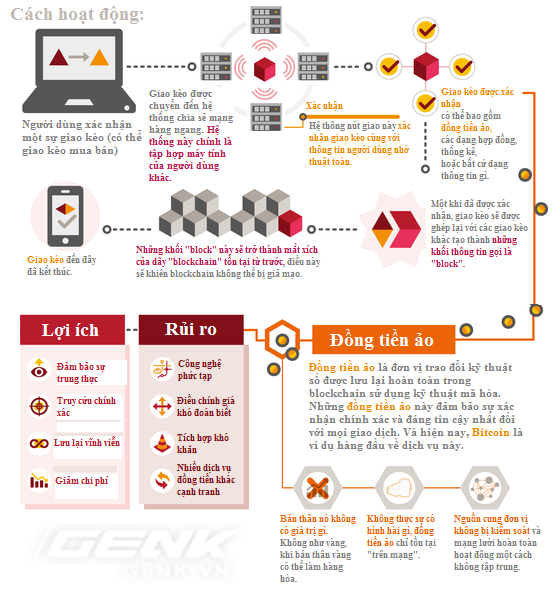
\includegraphics[width=0.7\linewidth]{C:/Users/kira/Desktop/howtowork}
	\caption{Cách hoạt động của chuỗi khối}
	\label{fig:howtowork}
\end{figure}
